

%%%%%%%%%%%%%%%%%%%%%%%%%%%%%%%%%%%
\subsection{Front-end Readout \& Buffering}
\label{sec:fd-daq-ltr}

\metainfo{Giles Barr \& Giovanna Miotto \& Brett Viren}

\begin{dunefigure}[Baseline Readout and Buffering]{fig:daq-readout-buffering-baseline}
  {Illustration of data flow for two out of 150 APAs in the \dword{sp}
    \dword{detmodule}. 
    The data is transmitted from the Cold Electronics WIBs to the
    \dwords{rce} which are part of the \dword{sp} DAQ \dword{fe}
    readout hardware. 
    The connections are such that each \dword{rce} receives data from
    the \dwords{femb} on one half of one APA face.
    The data and \dwords{trigprimitive} from the RCEs are received by
    a single FELIX board residing in a host computer. 
    The data is buffered into the \dword{ringbuffer} and the
    \dwords{trigprimitive} are processed and sent out as
    \dwords{trigcandidate} to the \dword{mtl}.
    Nominal (non-dump) \dwords{trigcommand} are delivered to the
    \dword{eb} which then queries the data selector on the appropriate
    FELIX host for the requested data.
    In the special case that a SNB candidate is detected the
    \dword{mtl} sends special dump command to the \dword{daqoob} which
    then informs all \dwords{rce} to dump what data they have buffered
    in local RAM and begin to stream subsequent data to local SSD
    storage.
    This dump is then sent out over Ethernet to a special SNB Event
    builder. 
    Both types of event builders finally save triggered data to file
    on the offline buffer disk.
    \fixme{This verbosity is maybe better in the text, and the figure needs work.}}  
  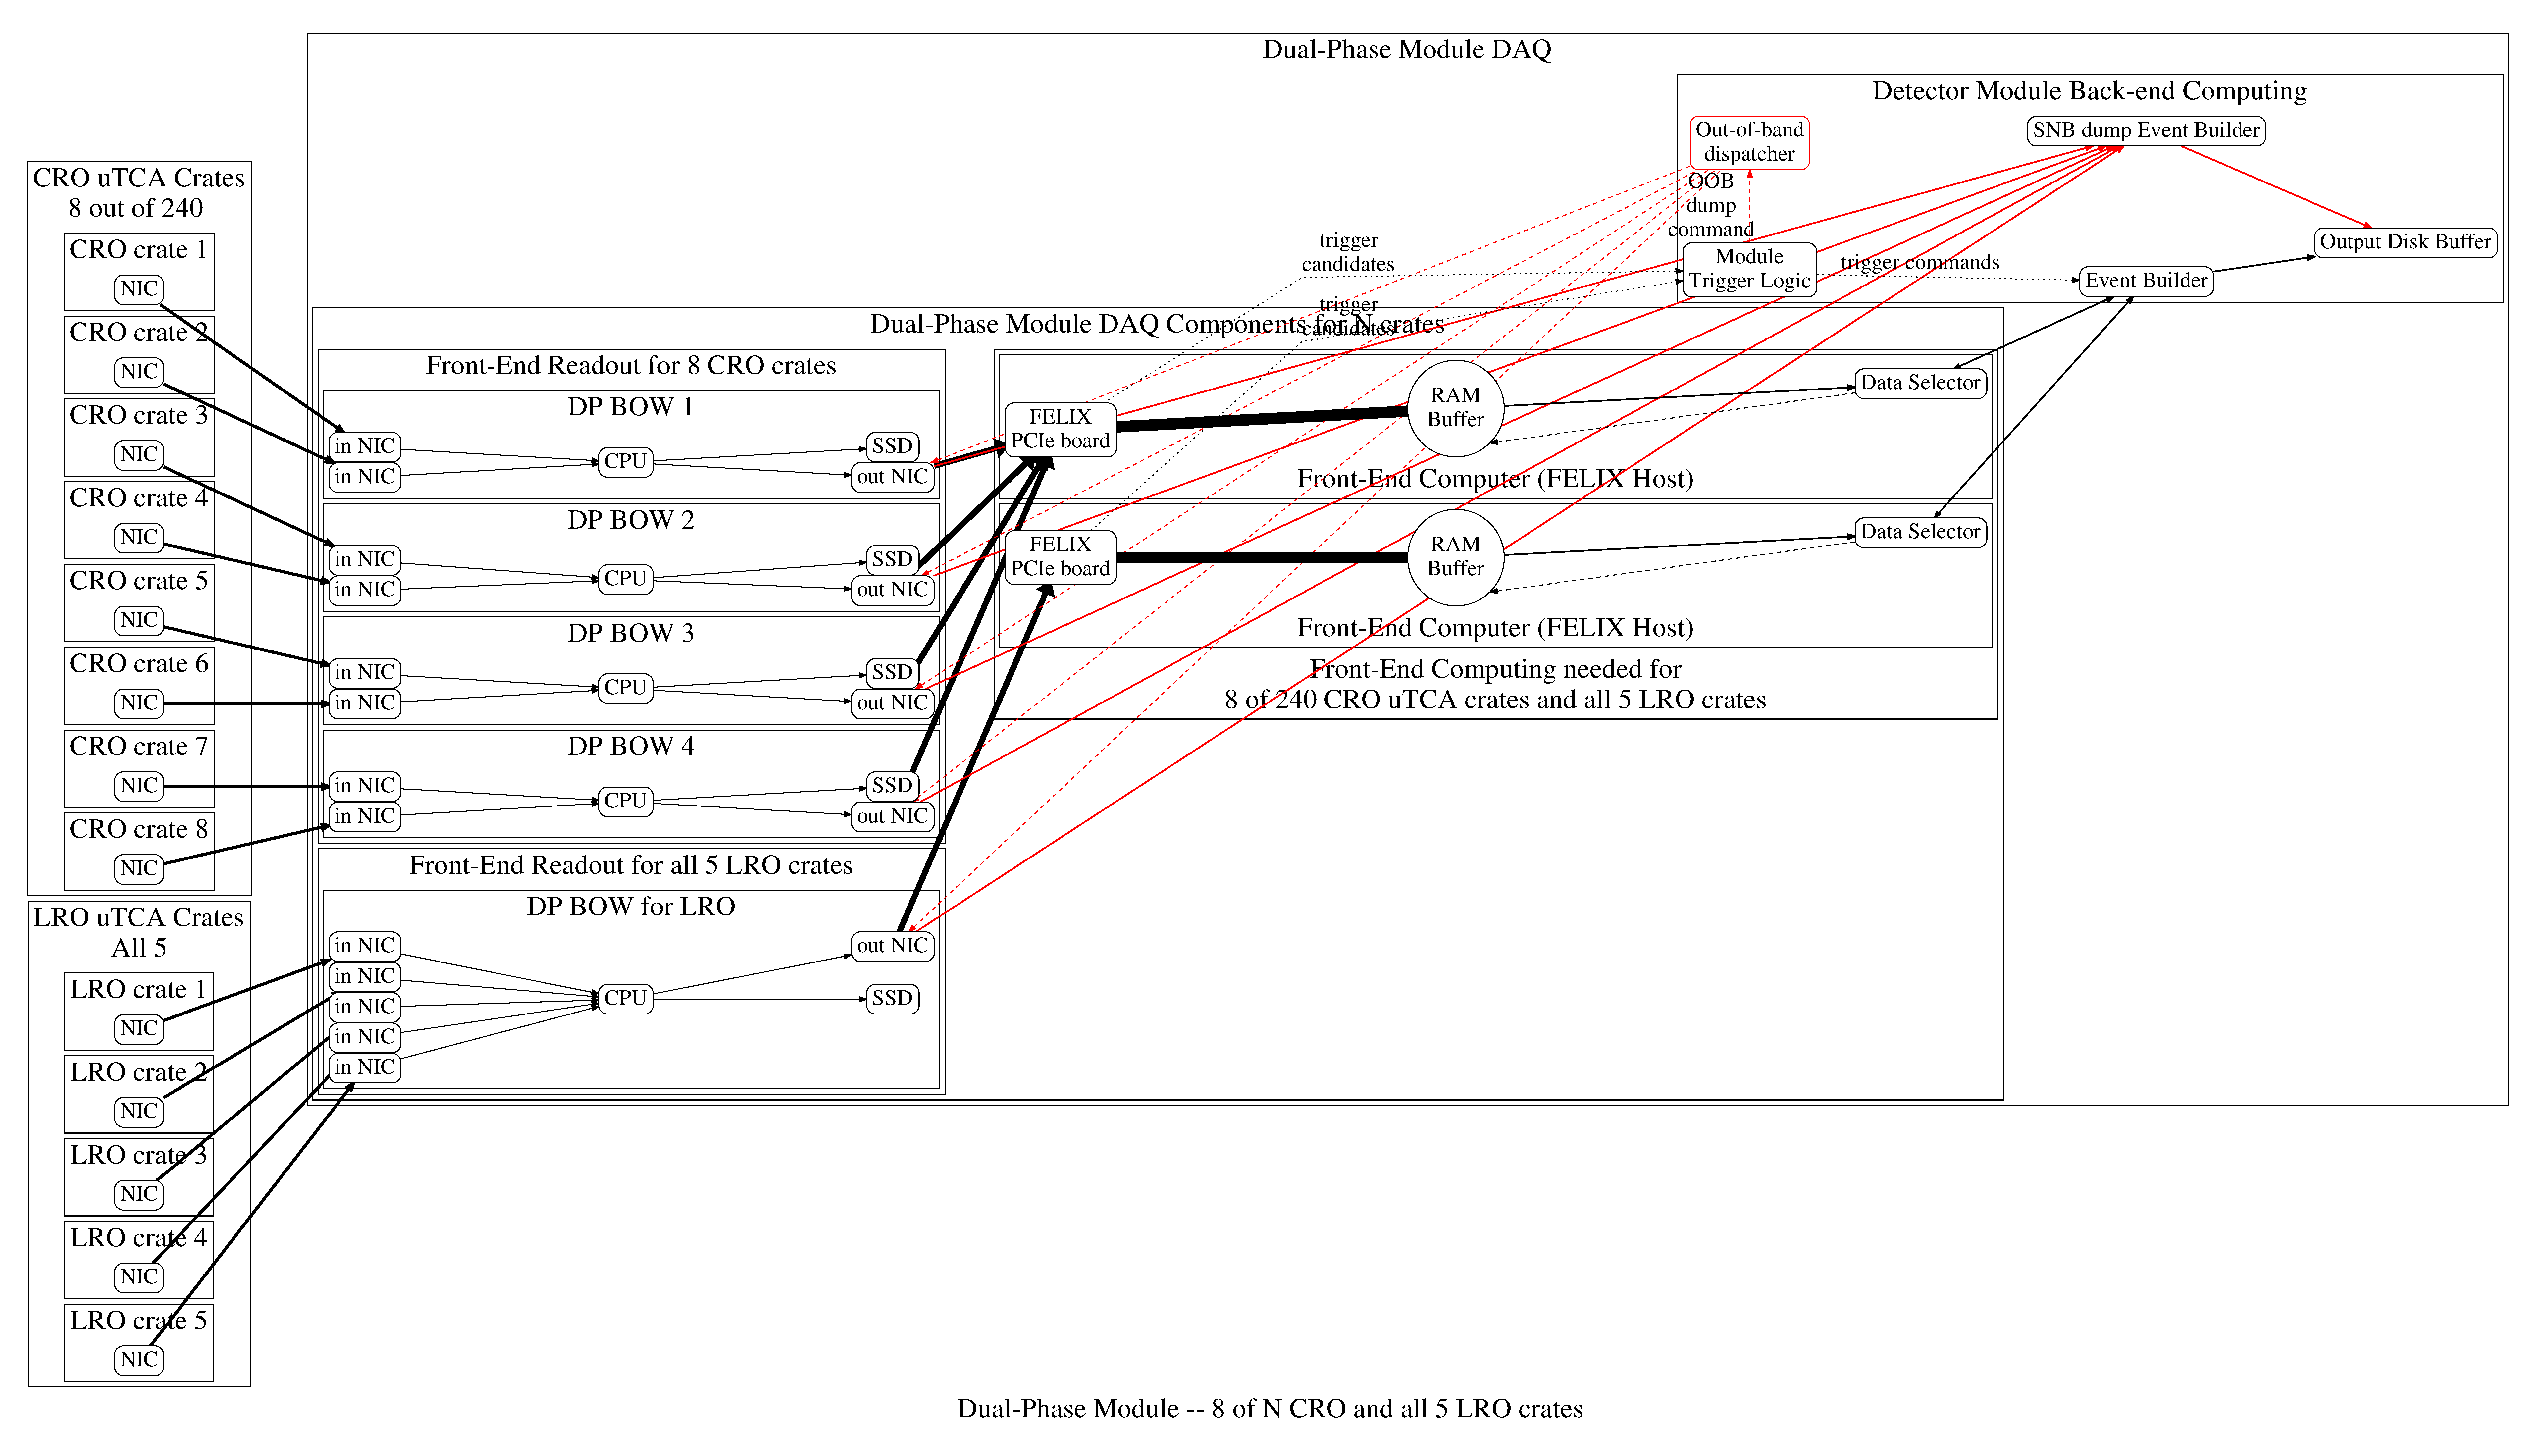
\includegraphics[width=0.8\textwidth]{daq-readout-buffering-baseline.pdf}%
\end{dunefigure}


Figure~\ref{fig:daq-readout-buffering-baseline} illustrates, in part,
the local readout and buffering and data flow in the context of one
\dword{fec}.  

In the \dword{sp} \dword{detmodule} DAQ there are two distributed RAM
storage systems which buffer the entire data flow. 
The \dword{ringbuffer}, which has a counterpart in the \dword{dp} DAQ
module, is distributed and resides in the \dwords{fec}, each
associated with two APAs. 
This buffer is sized to accommodate the data long enough to allow for
a nominal trigger decision to be made from the data itself.
Data flows into this buffer at a rate of about \SI{20}{\GB/\s} via the
\dword{felix} board which receives data from the \dwords{rce}
associated with two APAs. 
The \dword{felix} board performs DMA transfer to the system RAM. 
This transfer has been tested at \SI{10}{\GB/\s} by ATLAS in a PCIeV3
card. 
Current PCIeV4 and subsequent V5 are expected to each double the
throughput.
As that data is flowing through the buffer, the \dword{trigdecision}
process described below is ongoing.
A \dword{trigcommand} is interpreted by the \dword{eb} which issues
readout commands to an appropriate \dwords{daqds}. 
A \dword{daqds} is an agent running on the \dword{fec} which
executes the readout command by selecting the indicated portion of
data from the buffer and returning it to the \dword{eb} that issued
the request.

In the \dword{sp} DAQ module \dword{snb} triggering, buffering and
readout is managed separately from the nominal flow described above. 
The second distributed RAM buffer is to store the full data stream
long enough for a \dword{snb} \dword{trigcommand} to be formed and
distributed. 
The time for the number of \dword{snb} interactions throughout the
\dword{sp} \dword{detmodule} to rise above background rate is on order
\SI{1}{\s} and the nominal \dword{snb} \dword{readout window} is
\SI{10}{\s}. 
The \dword{snb} \dword{trigcommand} is issued to the \dword{daqoob} which
dispatches it to the 600 \dwords{rce}. 
Once received, each \dword{rce} will dump the portion of the requested
data which is already in the RAM buffer to local \dword{ssd} storage
and if the end of readout window is not yet reached it will stream the
data directly to the \dword{ssd} storage.
The rate to \dword{ssd} storage is \SI{2.5}{\GB/\s} which is
achievable with the fastest devices commonly available today. 
As high rate as this is, for a \SI{10}{\s} \dword{snb} readout window
this represents only \SI{25}{\GB} per \dword{snb} per \dword{rce}.
For a reasonable selection of thresholds it is expected that the
number of \dword{snb} triggers (almost all of which will be
false-positive) will be low enough to allow this data to reside on the
\dword{ssd} storage almost indefinitely and to be sent out of the DAQ
as a low-rate transfer.
This transfer will be performed using local network connections to a
special \dword{snb} \dword{eb}.
While the \dwords{rce} are dumping and transferring \dword{snb} dumps
they continue to supply the full data to the \dwords{fec} via the link
to the \dword{felix} boards.

